\textbf{COLUNI 2019 -- Questão 38}\par\medskip Veja a imagem abaixo e leia os textos a seguir:

% COLUNI-AUTO-FIGURES-BEGIN
\begin{figure}[htbp]
\centering
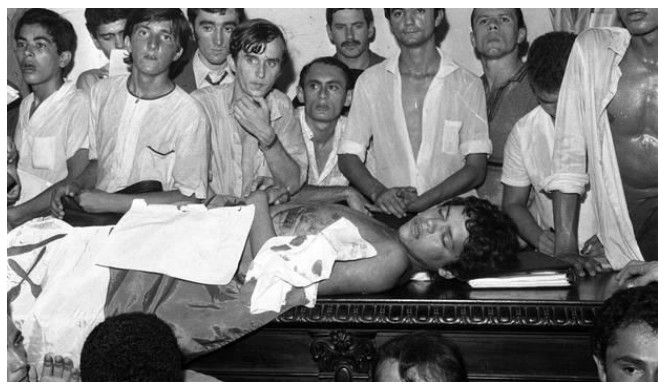
\includegraphics[width=0.95\linewidth]{static/simulados/coluni/figuras/2019/questao-38/figura-1.png}
\end{figure}
% COLUNI-AUTO-FIGURES-END

Estudantes velam o corpo de Edson Luís na Assembléia Legislativa do Rio: morto por um policial militar durante manifestação no Restaurante Calabouço, em 28/3/1968.

Há 50 anos, paraense de 18 anos levou um tiro durante movimento estudantil no restaurante Calabouço, no Rio. Onda de contestações políticas culmina com AI-5 do regime militar.

(Disponível em: <https://acervo.oglobo.globo.com/em-destaque/morte-do-estudante-edson-luis-em-1968-deflagra-protestos-no-pais-contra-ditadura-22470751#ixzz5SrWwyKcC>. Acesso em: 3 out. 2018.)

\textbf{Menino}

(Milton Nascimento)

Quem cala sobre teu corpo

Consente na tua morte

Talhada a ferro e fogo

Nas profundezas do corte

Que a bala riscou no peito

Quem cala morre contigo

Mais morto que estás agora

Relógio no chão da praça

Batendo, avisando a hora

Que a raiva traçou

No incêndio repetindo

O brilho de teu cabelo

Quem grita vive contigo.

(Disponível em: <http://www.letrasdemusicas.fm/milton-nascimento/menino>. Acesso em: 3 out. 2018.)

Em Dezembro de 1968, o Regime Militar decretou o Ato Institucional n° 5 em resposta a uma série de protestos da sociedade civil que aconteceram ao longo daquele ano, quando houve a morte do estudante secundarista Edson Luís de Lima Souto.

Assinale a alternativa que NÃO apresenta as características do período do Regime Militar, especialmente após a vigência do AI-5:
\begin{enumerate}
\item Censura e perseguição aos intelectuais como escritores e artistas, que tiveram que usar estratégias para
      denunciar as arbitrariedades do Regime, como na letra da música “Menino”, de Milton Nascimento.
\item Prisão de políticos de oposição, líderes sindicais, fechamento da União Nacional dos Estudantes (UNE) e
      a utilização da tortura, morte e desaparecimento de presos políticos.
\item Manutenção de eleições diretas para os poderes executivos e legislativo, o que garantia a ampla
      participação da população no processo político
\item Suspensão do direito de Habeas Corpus, que garantia aos cidadãos não serem presos arbitrariamente e
      poderem responder a um processo criminal em liberdade.
\end{enumerate}
